\subsection{Konstruowanie siatki}

\begin{frame}{Konstruowanie siatki}
  Dyskretyzacja zbioru punktów $R \bigcup S$
  $$ \left\{ \begin{array}{ll}
  (\overline{x}, \overline{y}) & \text{-- dowolny, ustalony punkt płaszczyzny} \\
  h > 0 & \text{-- rozmiar siatki (grid size)}
  \end{array} \right.$$
  \centerline{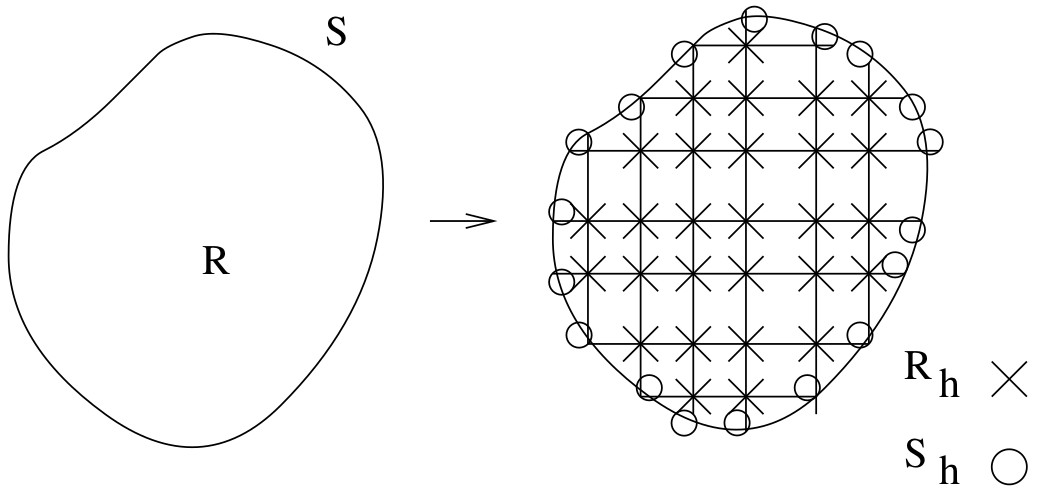
\includegraphics[width = \textwidth]{img/23/siatka}}
\end{frame}

\begin{frame}
  $$ \left\{ \begin{array}{ll}
  \text{zbiór punktów:} & \begin{array}{l} (\overline{x} + p \cdot h, \overline{y} + q \cdot h), \quad p,q = 0, \pm 1, \pm 2, \dots \\
    \rightarrow \text{zbiór punktów siatki płaskiej} \end{array}\\
  \text{zbiór linii:} & \left. \begin{array}{l}
    x = \overline{x} + p h \rightarrow \text{wertykalnych} \\
    y = \overline{y} + q h \rightarrow \text{horyzontalnych}
  \end{array} \right\} \begin{array}{l} \text{karta płaska} \\ \text{(planar lattice)} \end{array}
  \end{array} \right. $$
  $\rightarrow$ pokrywają całą płaszczyznę.
\end{frame}

\begin{frame}
  \begin{block}{}
    \begin{itemize}
      \item $R_h$ -- siatka wewnętrzna (interior grid): te punkty siatki, które należą do $R$
      \item $S_h^*$ -- punkty wspólne karty płaskiej i brzegu $S$
      \item $G_h^* = R_h \bigcup S_h^*$
      \item 4 sąsiedzi $(x,y) \in R_h \rightarrow$ 4 punkty $\in G_h^*$ najbliższe $(x,y)$  \\
w 4 kierunkach
      \item $G_h$ -- podzbiór $G_h^*$ zawierający każdy punkt $R_h$ i 4 jego sąsiadów
      \item Brzeg siatki $S_h = G_h - R_h$
    \end{itemize}
  \end{block}
\end{frame}
